\documentclass[12pt, letterpaper]{article}
% --- PAQUETES DE IDIOMA Y CODIFICACIÓN ---
\usepackage[spanish, es-tabla]{babel}
\usepackage[utf8]{inputenc}
\usepackage[T1]{fontenc}
% --- FORMATO DE PÁGINA Y FUENTE (Instrucción: 2cm, Arial 12, Interlineado 1.15) ---
\usepackage[margin=2cm]{geometry}
\usepackage[scaled]{helvet}
\renewcommand\familydefault{\sfdefault}
\usepackage{setspace}
\setstretch{1.15}
% --- PAQUETES GRÁFICOS Y TABLAS ---
\usepackage{graphicx}
\usepackage{booktabs}
\usepackage[table]{xcolor}
\usepackage{float}
\usepackage{caption}
\usepackage{csquotes}
\usepackage{enumitem}
\usepackage{multirow}
% --- ENCABEZADO Y PIE DE PÁGINA ---
\usepackage{fancyhdr}
\pagestyle{fancy}
\fancyhf{}
\renewcommand{\headrulewidth}{0.4pt}
\fancyhead[L]{\small CD1100 Desafíos de Innovación en Ingeniería y Ciencias}
\fancyhead[R]{\small pág. \thepage}
% --- BIBLIOGRAFÍA APA 7 ---
\usepackage[backend=biber, style=apa]{biblatex}
\addbibresource{library.bib}
% ======================================================================
\begin{document}

% --- PORTADA ---
\begin{titlepage}
    \thispagestyle{empty}
    \centering
    \vspace*{0.5cm}
    
\includegraphics[width=0.22\textwidth]{img/departamentos/uchile.pdf}
    \hspace{1.5cm}
    
\includegraphics[width=0.28\textwidth]{img/departamentos/fcfm.pdf}
    \par\vspace{1cm}
    {\scshape\large Facultad de Ciencias Físicas y Matemáticas\par}
    {\scshape\normalsize Departamento de Ingeniería Mecánica / Eléctrica\par}
    \vfill
    {\large Reporte Hito 1\par}
    \vspace{0.4cm}
    {\huge\bfseries Exploración del Desafío:\\[0.2cm]
    Contaminación Subsuperficial\\[0.2cm]
    en Playas Chilenas\par}
    \vspace{0.5cm}
    {\large Desafíos de Innovación en Ingeniería y Ciencias\par}
    \vfill
    \begin{table}[H]
        \centering
        \renewcommand{\arraystretch}{1.6}
        \begin{tabular}{|p{0.88\textwidth}|}
            \hline
            \rowcolor[HTML]{4F81BD} \textcolor{white}{\textbf{EQUIPO:}} \\ \hline
            \textbf{Sección:} 1 \\
            \textbf{Número y nombre del equipo:} Grupo 3 \\
            \textbf{Fecha de entrega:} 21 de abril de 2026 \\ \hline
            \textbf{Nombre de los Integrantes del Equipo:} \\
            1. Felipe Colli Olea \quad 2. Agustín Concha \quad 3. Benjamín Bascuñán \\
            4. Diego Alvarado \quad 5. Joaquín Pérez \\ \hline
        \end{tabular}
    \end{table}
    \vspace{0.4cm}
    \textbf{Profesor:} María Pino\par
    \vfill
    Santiago, Chile \\ Abril de 2026
\end{titlepage}

% --- ÍNDICE ---
\newpage
\thispagestyle{empty}
\pagenumbering{roman}
\tableofcontents
\newpage

% --- INICIO CUERPO ---
\pagenumbering{arabic}
\setcounter{page}{1}

% ==========================================================
\section*{Resumen Ejecutivo}
\addcontentsline{toc}{section}{Resumen Ejecutivo}
% ==========================================================

Las playas chilenas enfrentan un problema crítico de contaminación que va más allá de lo visible. 
Si bien la limpieza municipal se enfoca en los residuos superficiales, una vasta cantidad de 
macroplásticos, colillas de cigarro, vidrios y envases permanece enterrada bajo la arena, 
representando un peligro físico constante para residentes y turistas. 
En 2024, se recolectaron 86 toneladas de basura en las costas del país, generando pérdidas 
económicas estimadas en US\$60,7 millones \parencite{oceana_2026}.

Este reporte documenta la fase de diagnóstico e investigación del desafío de contaminación 
subsuperficial, centrado en playas como El Tabo. A través de una revisión del estado del arte, 
observación de campo planificada, entrevistas a usuarios y herramientas de empatía, se valida 
la existencia de una brecha: la limpieza manual y las regulaciones vigentes son insuficientes 
para extraer los residuos que se entierran progresivamente en la arena. 
El problema se define mediante la sintaxis aprendida en el curso: 
\textit{Residentes y turistas de playas chilenas necesitan playas libres de basura enterrada, 
debido al riesgo de accidentes por cortes y degradación ambiental, puesto que la limpieza 
manual no logra extraer macroplásticos subsuperficiales.}

Las conclusiones confirman la factibilidad de concebir soluciones de carácter mecánico para 
abordar este problema, y se identifican los Objetivos de Desarrollo Sostenible (ODS) 14 
(\textit{Vida Submarina}) y 11 (\textit{Ciudades y Comunidades Sostenibles}) como marcos 
de referencia pertinentes.

% ==========================================================
\newpage
\section{Introducción}
% ==========================================================

Chile posee una costa de aproximadamente 6.500 km de extensión, lo que la convierte 
en uno de los litorales más largos del mundo. Sin embargo, esta riqueza natural está 
siendo gravemente deteriorada por la acumulación de residuos sólidos en las playas del 
país \parencite{bravo_2009}. Cada temporada estival, el aumento masivo de visitantes 
agrava la situación: se depositan plásticos, colillas, vidrios y envases que, con el paso 
del tiempo, se entierran bajo la arena y quedan fuera del alcance de la limpieza 
convencional \parencite{radio_uchile_2025}.

La problemática no se limita al plano estético. Los residuos enterrados representan un 
peligro físico directo para quienes usan la playa descalzos, afectan a la fauna costera 
y degradan los ecosistemas marinos de manera silenciosa \parencite{oceana_2026}. 
A pesar de la existencia de legislación como las Leyes 21.100, 21.368 y 21.413 que 
restringen el uso de plásticos de un solo uso, la fiscalización es insuficiente y los 
métodos actuales de limpieza ---fundamentalmente manuales--- no logran abordar la 
capa subsuperficial de contaminación.

A nivel internacional, países como Alemania, España y Estados Unidos utilizan maquinaria 
especializada de cribado para limpiar sus playas de forma mecánica y profunda 
\parencite{beachtech_2020}. Chile, en cambio, carece de soluciones tecnológicas adaptadas 
a su contexto, escala y recursos.

\subsection{Objetivos}

\textbf{Objetivo general:} Investigar y caracterizar la problemática de contaminación 
subsuperficial en playas chilenas, identificando sus causas, actores involucrados 
y la brecha existente en los métodos de limpieza actuales.

\textbf{Objetivos específicos:}
\begin{enumerate}
    \item Caracterizar los tipos y distribución de residuos presentes en la arena de 
    playas chilenas, con foco en macroplásticos.
    \item Identificar las necesidades y percepciones de los usuarios del borde costero 
    mediante entrevistas y herramientas empáticas.
    \item Analizar el estado del arte de soluciones existentes a nivel nacional e 
    internacional para determinar las brechas tecnológicas relevantes.
    \item Establecer los fundamentos éticos y de sostenibilidad que enmarcan el problema.
\end{enumerate}

% ==========================================================
\newpage
\section{Desarrollo}
% ==========================================================

\subsection{Síntesis del Estado del Arte}

La investigación bibliográfica revela que la contaminación en las costas chilenas 
es un problema de magnitud industrial. Según un estudio reciente, en la temporada 
2024 se recolectaron 86 toneladas de basura en playas del país, compuestas principalmente 
por plásticos (61\%), colillas de cigarro (18\%) y vidrio (7\%), generando pérdidas 
económicas estimadas en US\$60,7 millones \parencite{oceana_2026}. 
Investigaciones previas ya advertían sobre la acumulación crónica de residuos 
antropogénicos en el Pacífico suroriental \parencite{bravo_2009}.

Frente a este panorama, el enfoque actual combina limpieza manual y regulaciones legales, 
ambos mecanismos que han demostrado ser insuficientes sin una fiscalización efectiva 
\parencite{radio_uchile_2025}. La comparación con soluciones internacionales evidencia 
una brecha significativa: mientras países desarrollados emplean maquinaria de cribado 
que tamiza la arena en profundidad \parencite{beachtech_2020}, en Chile predomina el 
trabajo voluntario y manual, que por definición solo alcanza la superficie visible.

El análisis de referentes de robótica aplicada a limpieza de playas \parencite{publimetro_2024} 
confirma que los prototipos existentes presentan limitaciones importantes: algunos requieren 
supervisión humana constante, otros son autónomos pero carecen de capacidad de filtrado 
físico, y los más especializados están diseñados para un solo tipo de residuo. 
Esto valida que existe un vacío tecnológico real: ninguna solución actual combina 
autonomía con tamizado eficiente de macroplásticos de distinto tamaño 
\parencite{garcia_dominguez_2021}.

\begin{figure}[H]
    \centering
    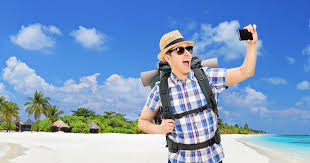
\includegraphics[width=0.62\textwidth]{img/5.jpg}
    \caption{Costa chilena con acumulación visible de residuos sólidos. Fuente: Imagen referencial.}
    \label{fig:costa_sucia}
\end{figure}

\subsection{Definición de la Problemática}

A partir de la investigación bibliográfica, la observación planificada y el análisis 
empático, el problema se define con la siguiente sintaxis:

\vspace{0.5cm}
\begin{center}
\fboxsep=10pt
\fbox{\parbox{0.85\textwidth}{
\centering
\textbf{Residentes y turistas de playas chilenas} (Usuario) \textbf{+} necesitan 
playas libres de basura enterrada (Necesidad) \textbf{+} debido al riesgo de accidentes 
por cortes y degradación ambiental (Síntoma) \textbf{+} puesto que la limpieza manual 
no logra extraer macroplásticos subsuperficiales (Hallazgo).
}}
\end{center}
\vspace{0.5cm}

Los usuarios afectados son múltiples y con distintos roles: residentes costeros permanentes, 
turistas nacionales e internacionales, trabajadores de aseo municipal, salvavidas y 
vendedores ambulantes. Cada uno experimenta el problema desde una perspectiva diferente, 
pero todos comparten la exposición a un entorno degradado.

\begin{figure}[H]
    \centering
    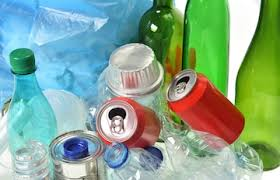
\includegraphics[width=0.62\textwidth]{img/4.jpg}
    \caption{Residuos sólidos sobre la arena, representando riesgo físico para los usuarios. Fuente: Imagen referencial.}
    \label{fig:basura_playa}
\end{figure}

\subsection{Metodología de Investigación}

La recopilación de información se estructuró en tres ejes complementarios:

\textbf{Revisión bibliográfica:} Se consultaron bases de datos académicas, organismos 
gubernamentales (DIRECTEMAR, Subsecretaría del Medio Ambiente) e informes de 
organizaciones ambientales como Oceana Chile y Científicos de la Basura \parencite{araya_2026}. 
El foco estuvo en estadísticas nacionales de residuos costeros, legislación vigente y 
comparación de métodos de limpieza internacionales.

\textbf{Entrevista de diagnóstico:} Se realizó una entrevista semiestructurada a Ana Jer 
(56 años, residente de El Tabo desde 2018, a 10 minutos caminando del mar), cuya 
transcripción completa se incluye en el Anexo~\ref{anexo:entrevista}. 
Sus respuestas validaron empíricamente los hallazgos bibliográficos: la municipalidad 
limpia diariamente pero no da abasto, los vendedores ambulantes siguen usando envases 
plásticos a pesar de las leyes, y los turistas reducen su intención de regresar por el 
mal estado de las playas.

\textbf{Observación de campo planificada:} Se diseñó un protocolo estructurado de 
salida a terreno (Anexo~\ref{anexo:campo}), orientado a una playa cercana a la Región 
Metropolitana (El Tabo, Algarrobo o Cartagena). El protocolo incluye recorridos 
sistemáticos, conteo de residuos por tipo, fotografías georreferenciadas y entrevistas 
breves in situ.

\subsection{Análisis AEIOU y Hallazgos Empáticos}

La aplicación de la metodología AEIOU permitió organizar sistemáticamente las 
observaciones del entorno costero:

\begin{table}[H]
\centering
\caption{Matriz AEIOU -- Observación del entorno costero.}
\label{tab:aeiou}
\renewcommand{\arraystretch}{1.4}
\begin{tabular}{|p{2.8cm}|p{10.5cm}|}
\hline
\rowcolor[HTML]{4F81BD}\textcolor{white}{\textbf{Dimensión}} & \textcolor{white}{\textbf{Hallazgos}} \\ \hline
\textbf{Actividades} & Limpieza manual por voluntarios y trabajadores municipales; uso recreativo por turistas y residentes. \\ \hline
\textbf{Entornos} & Borde costero chileno; arena superficial y subsuperficial; zonas de alta y baja concurrencia. \\ \hline
\textbf{Interacciones} & Descuido de turistas con residuos; esfuerzo de voluntarios limitado a superficie visible. \\ \hline
\textbf{Objetos} & Botellas plásticas, colillas de cigarro, vidrios rotos, envases de comercio ambulante, bolsas plásticas. \\ \hline
\textbf{Usuarios} & Residentes, turistas, vendedores ambulantes, trabajadores de aseo, salvavidas. \\ \hline
\end{tabular}
\end{table}

El cruce con el Mapa de Empatía (Anexo~\ref{anexo:empatia}) reveló que los usuarios 
perciben frecuentemente las playas como lugares contaminados y peligrosos. 
La entrevistada Ana Jer expresó que siente que es desagradable e inseguro caminar 
descalzo por la playa, y que recoge basura del suelo por iniciativa propia al observar 
la inacción colectiva.

\begin{figure}[H]
    \centering
    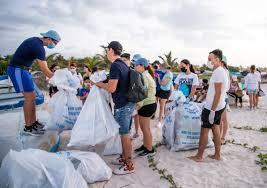
\includegraphics[width=0.60\textwidth]{img/1.jpg}
    \caption{Voluntarios realizando limpieza manual en playa. Fuente: Imagen referencial.}
    \label{fig:voluntarios}
\end{figure}

\subsection{Estudio Ético del Problema}

Todo proyecto de ingeniería que interviene en un espacio público y natural debe considerar 
sus implicancias éticas. En este caso, se identifican tres dimensiones principales:

\textbf{Dignidad laboral:} La limpieza manual de playas expone a los trabajadores 
municipales y voluntarios a tareas físicamente exigentes y potencialmente peligrosas 
(contacto con vidrios, jeringas u otros residuos corto-punzantes). Una solución 
mecanizada debe concebirse como complemento que dignifique ---no reemplace--- 
el trabajo humano.

\textbf{Protección del ecosistema:} Cualquier intervención en la arena debe 
garantizar que no se dañe la fauna bentónica ni se altere la estructura del sedimento 
costero de manera irreversible. La profundidad y frecuencia del tamizado debe 
estudiarse en coordinación con biólogos marinos.

\textbf{Equidad de acceso:} Las playas son espacios públicos. Las soluciones 
propuestas deben ser accesibles para municipios con presupuestos limitados y no 
deben generar una brecha entre comunas con distintos niveles de recursos.

\subsection{Etapas del Proceso de Innovación}

El equipo ha seguido las siguientes fases hasta el momento:

\begin{enumerate}
    \item \textbf{Exploración del desafío:} Selección de la problemática de 
    contaminación costera a partir de observaciones cotidianas y noticias recientes.
    \item \textbf{Investigación y caracterización:} Revisión del estado del arte, 
    análisis de legislación vigente y estudio de referentes internacionales.
    \item \textbf{Empatía con usuarios:} Construcción de mapa de empatía y 
    entrevista de diagnóstico a residente costera.
    \item \textbf{Definición del problema:} Síntesis de hallazgos en la sintaxis 
    Usuario + Necesidad + Síntoma + Hallazgo.
    \item \textbf{Próximos pasos:} Ejecución de la observación de campo planificada 
    para cuantificar los hallazgos y refinar la definición del problema.
\end{enumerate}

\begin{figure}[H]
    \centering
    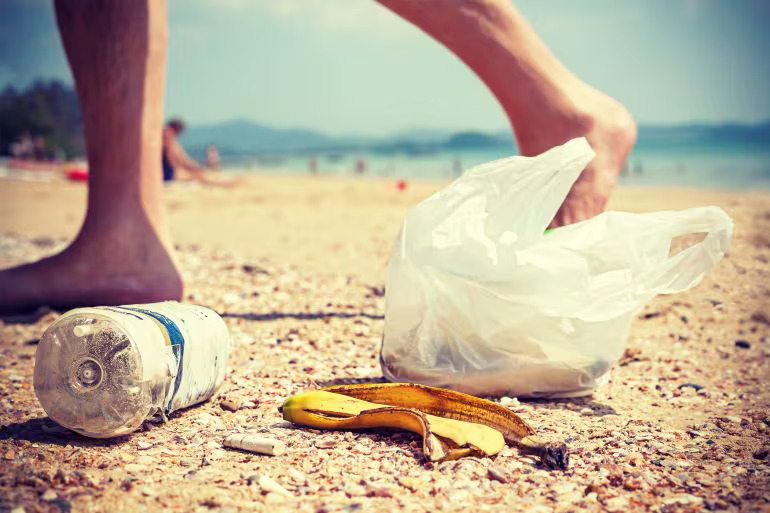
\includegraphics[width=0.55\textwidth]{img/3.jpg}
    \caption{Tipos de residuos sólidos encontrados en playas: botellas, latas y envases plásticos. Fuente: Imagen referencial.}
    \label{fig:residuos}
\end{figure}

% ==========================================================
\newpage
\section{Conclusiones}
% ==========================================================

La investigación realizada confirma que la contaminación subsuperficial de playas chilenas 
es un problema grave, recurrente y actualmente sin solución efectiva. La limpieza manual 
y la legislación vigente son necesarias pero insuficientes: los macroplásticos continúan 
enterrándose en la arena, acumulando impactos físicos, económicos y ecológicos de 
forma silenciosa.

\textbf{Síntesis del problema:} El problema radica en que los métodos de limpieza 
actuales operan exclusivamente en la superficie visible de la arena, ignorando la capa 
subsuperficial donde se acumulan progresivamente residuos de alto riesgo para los usuarios.

\textbf{Atractivo del problema:} Se trata de un problema con alta relevancia social 
(afecta a millones de visitantes y residentes costeros cada año), económica 
(US\$60,7 millones en pérdidas documentadas \parencite{oceana_2026}) y ambiental 
(degradación de ecosistemas marinos únicos de Chile).

\textbf{Conexión con ODS:} El problema se enmarca directamente en el ODS 14 
(\textit{Vida Submarina}), al buscar reducir la contaminación marina, y en el ODS 11 
(\textit{Ciudades y Comunidades Sostenibles}), al promover espacios públicos limpios 
y seguros para todas las personas.

\textbf{Factibilidad de soluciones:} Sí se considera factible concebir y diseñar 
soluciones para abordar este problema. La comparación internacional demuestra que 
el cribado mecánico es técnicamente viable \parencite{canon_2021}, y el análisis de 
referentes existentes \parencite{garcia_dominguez_2021} permite identificar con 
claridad qué aspectos aún no han sido resueltos adecuadamente.

\textbf{Aprendizajes del equipo:} Durante esta fase aprendimos que un problema 
aparentemente simple (la basura en la playa) esconde una complejidad sistémica 
significativa: involucra actores diversos, dinámicas de comportamiento difíciles de 
cambiar solo con legislación, y una dimensión técnica concreta que los métodos 
manuales no pueden resolver. La metodología de empatía y el análisis AEIOU fueron 
fundamentales para comprender el problema desde la perspectiva del usuario real, 
no solo desde los datos.

\textbf{Plan de avance:} El siguiente paso es ejecutar la observación de campo 
planificada en una playa de la zona central de Chile, con el objetivo de cuantificar 
los tipos y profundidades de residuos, validar los hallazgos de la entrevista y 
establecer los requerimientos concretos que deberá cumplir cualquier solución al problema.

\textbf{Alcances y limitaciones éticas:} Es importante considerar que toda intervención 
mecánica en el ecosistema de playa debe ser evaluada en términos de su impacto sobre 
la fauna bentónica y la estructura del sedimento. Asimismo, cualquier solución debe 
ser accesible para municipios con distintas capacidades económicas, para no reproducir 
desigualdades territoriales.

% ==========================================================
\newpage
\printbibliography[title={Referencias Bibliográficas}]
\addcontentsline{toc}{section}{Referencias Bibliográficas}

% ==========================================================
\newpage
\appendix
\section{Mapa de Empatía}
\label{anexo:empatia}
% ==========================================================

\textbf{Usuario: Ana Jer, 56 años. Residente de El Tabo desde 2018. 
Vive a aproximadamente 10 minutos caminando del borde costero.}

\begin{table}[H]
\centering
\caption{Mapa de Empatía -- Ana Jer.}
\renewcommand{\arraystretch}{1.6}
\begin{tabular}{|p{3.5cm}|p{10cm}|}
\hline
\rowcolor[HTML]{4F81BD}\textcolor{white}{\textbf{Dimensión}} & \textcolor{white}{\textbf{Contenido}} \\ \hline
\textbf{¿Qué ve?} & Playa contaminada por colillas y macroplásticos. Personas disfrutando sin importarles el entorno. \\ \hline
\textbf{¿Qué oye?} & Quejas de otras personas por el mal estado de la playa; comentarios sobre la falta de esfuerzo contra la contaminación. \\ \hline
\textbf{¿Qué piensa y siente?} & Siente que es desagradable y peligroso ir descalzo. Piensa que las personas deben hacerse responsables de su basura. \\ \hline
\textbf{¿Qué hace?} & Recoge basura del suelo para tirarla en contenedores. Trata de no contaminar. \\ \hline
\textbf{Dolores} & Exposición a vidrios y objetos cortantes al caminar por la arena; sensación de impotencia ante la inacción colectiva. \\ \hline
\textbf{Ganancias} & Valora la limpieza, el cuidado y la protección de la playa como espacio público compartido. \\ \hline
\end{tabular}
\end{table}

% ==========================================================
\section{Matriz AEIOU Extendida}
\label{anexo:aeiou}
% ==========================================================

\begin{figure}[H]
    \centering
    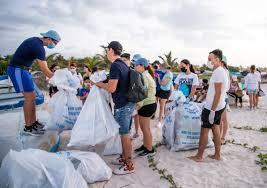
\includegraphics[width=0.55\textwidth]{img/1.jpg}
    \caption{Voluntarios realizando limpieza en playa. Fuente: Imagen referencial.}
\end{figure}

\begin{figure}[H]
    \centering
    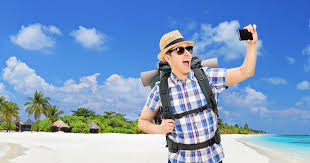
\includegraphics[width=0.55\textwidth]{img/5.jpg}
    \caption{Costa chilena con acumulación de residuos. Fuente: Imagen referencial.}
\end{figure}

\begin{figure}[H]
    \centering
    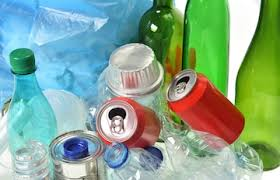
\includegraphics[width=0.55\textwidth]{img/4.jpg}
    \caption{Residuos visibles sobre la arena. Fuente: Imagen referencial.}
\end{figure}

\begin{figure}[H]
    \centering
    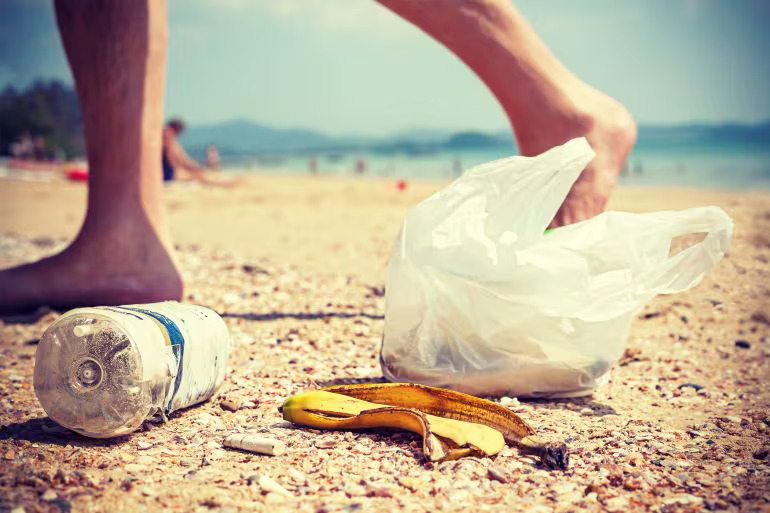
\includegraphics[width=0.55\textwidth]{img/3.jpg}
    \caption{Tipos de residuos: botellas, latas y envases plásticos. Fuente: Imagen referencial.}
\end{figure}

\begin{figure}[H]
    \centering
    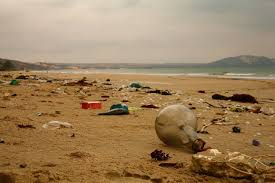
\includegraphics[width=0.55\textwidth]{img/2.jpg}
    \caption{Turista en playa chilena. Fuente: Imagen referencial.}
\end{figure}

% ==========================================================
\section{Planificación de la Observación de Campo}
\label{anexo:campo}
% ==========================================================

Esta planificación detalla el protocolo estructurado para la salida a terreno, 
basada en los requerimientos de investigación del proyecto.

\subsection*{¿Qué se va a observar?}
\begin{itemize}
    \item Tipo y cantidad de basura presente en la arena 
    (colillas, vidrios, plásticos, latas, etc.).
    \item Profundidad aproximada a la que se entierra la basura visible.
    \item Cómo se realiza actualmente la limpieza de la playa 
    (personas, máquinas, frecuencia).
    \item Uso de la playa: actividades principales y zonas más concurridas.
\end{itemize}

\subsection*{¿Cómo se va a observar?}
\begin{itemize}
    \item Observación no participante, con registro estructurado 
    en una planilla de conteo de residuos.
    \item Recorridos definidos a lo largo del tramo de playa, 
    anotando hallazgos cada ciertos metros.
    \item Entrevistas breves semiestructuradas a usuarios y 
    trabajadores de la playa.
\end{itemize}

\subsection*{¿Cuándo se va a observar?}
\begin{itemize}
    \item Un fin de semana a definir, idealmente en horario de tarde 
    (aprox. 15:00--17:00 h).
    \item Duración total estimada: 2--3 horas en terreno.
\end{itemize}

\subsection*{¿Con qué se va a observar?}
\begin{itemize}
    \item Celulares para fotografías, videos y grabación de entrevistas.
    \item Planillas impresas para notas de campo y conteo de residuos.
    \item Materiales básicos de escritura.
\end{itemize}

\subsection*{¿Dónde se va a observar?}
\begin{itemize}
    \item Playa cercana a la Región Metropolitana: El Tabo, 
    Algarrobo o Cartagena.
    \item Tramo delimitado de 200--300 metros lineales para el catastro.
\end{itemize}

\subsection*{¿Quiénes estarán presentes?}
Los 5 integrantes del equipo, con roles definidos:
\begin{itemize}
    \item 1 encargado/a de notas de campo.
    \item 1 encargado/a de fotografías y videos.
    \item 1--2 encargados/as de realizar entrevistas.
    \item 1 encargado/a de registrar conteos en la planilla.
\end{itemize}

\subsection*{Objetivos de la observación}
\begin{itemize}
    \item Caracterizar los tipos de residuos y su distribución en la arena.
    \item Entender con qué frecuencia y métodos se limpia actualmente la playa.
    \item Identificar necesidades concretas que guíen la siguiente etapa del proyecto.
\end{itemize}

\subsection*{Criterios de éxito}
\begin{itemize}
    \item Completar el recorrido del tramo delimitado.
    \item Obtener al menos 50 observaciones de residuos por tipo.
    \item Realizar al menos 5 entrevistas breves a usuarios y/o trabajadores.
\end{itemize}

\subsection*{Limitaciones previstas}
\begin{itemize}
    \item La observación es específica a una fecha y lugar; 
    no es representativa de todas las playas de Chile.
    \item Falta de instrumentos para medir con precisión 
    la profundidad de enterramiento.
    \item Posible negativa de personas a ser entrevistadas o fotografiadas.
\end{itemize}

% ==========================================================
\section{Transcripción de Entrevista de Diagnóstico}
\label{anexo:entrevista}
% ==========================================================

\textbf{Información de la entrevistada:}\\
Nombre: Ana Jer. Edad: 56 años. Residencia: El Tabo, desde 2018.\\
Cercanía a la costa: Aproximadamente 10 minutos caminando.

\vspace{0.5cm}

\begin{enumerate}
    \item \textbf{¿Qué tipo de basura ves más en la arena?}\\
    ``Botellas plásticas y colillas de cigarro. Durante la pandemia 
    se veían muchas mascarillas.''

    \item \textbf{¿Quién limpia esta playa y cada cuánto?}\\
    ``La municipalidad se encarga diariamente, pero no da abasto 
    con la cantidad de basura que se forma. ¡Mientras más escarbas, más sale!''

    \item \textbf{¿Crees que la basura aleja a los turistas?}\\
    ``Sí, he escuchado turistas decir que no volverían por malos ratos; 
    mucha gente se entierra vidrios.''

    \item \textbf{¿Sientes que se fiscalizan las leyes contra los plásticos?}\\
    ``A nivel de comercio en negocios sí, pero los vendedores ambulantes 
    siguen trayendo comida en envases plásticos.''

    \item \textbf{¿Aumenta mucho la basura con la llegada de turistas?}\\
    ``Sí, durante el verano se ve mucha más basura, ya que aumenta 
    la cantidad de gente que transita y que se hospeda en la zona.''
\end{enumerate}

\end{document}
